\section{Results}

We report closure rates across the 20-cell DOE on the 150-function core dataset, comprising 5{,}890 measurement rows (150 mono samples $\times$ 3 paths $\times$ 6 mono cells $+$ 75 hetero samples $\times$ 3 paths $\times$ 11 hetero cells $+$ 75 null samples $\times$ 3 paths $\times$ 3 null cells). Results are organised by research question. Every closure rate reported here uses the strict two-signal validity policy of Eq.~\ref{eq:valid1}--\ref{eq:valid3} with default thresholds $\tau_1 = \tau_2 = \tau_3 = 0$ and $\rho = 3$; Section~5.6 confirms every headline finding survives alternative threshold choices.

\subsection{Overall closure rates per cell and path}

Table~\ref{tab:closure_rate_matrix} and Fig.~\ref{fig:closure_heatmap} present the mean closure rate for every cell $\times$ path combination. Three high-level patterns emerge.

\needspace{22\baselineskip}

\noindent
\centering
\begin{tabular}{@{}lccc@{}}
\toprule
Cell & Path 1 & Path 2 & Path 3 \\
\midrule
M1   & 0.577~(75) & 0.367~(45) & 0.245~(61) \\
M2   & 0.769~(63) & 0.547~(71) & 0.185~(81) \\
M3   & \textbf{0.900}~(100) & 0.647~(90) & 0.208~(105) \\
M4   & 0.856~(116) & 0.647~(87) & \textbf{0.282}~(109) \\
M5   & 0.781~(98) & 0.533~(69) & 0.261~(80) \\
M6   & 0.862~(108) & 0.647~(86) & 0.219~(100) \\
\midrule
H1   & 0.854~(64) & \textbf{0.674}~(57) & 0.194~(56) \\
H2   & 0.862~(35) & 0.613~(40) & 0.185~(40) \\
H3   & 0.787~(50) & 0.627~(42) & 0.174~(29) \\
H4   & 0.862~(60) & 0.453~(30) & 0.199~(50) \\
H5   & 0.811~(50) & 0.667~(47) & 0.218~(37) \\
H6   & 0.882~(53) & 0.600~(41) & 0.184~(49) \\
H7   & 0.872~(57) & 0.600~(42) & 0.200~(53) \\
H8   & 0.846~(53) & 0.600~(43) & 0.260~(54) \\
H9   & 0.881~(54) & 0.627~(46) & 0.202~(55) \\
H10  & 0.764~(22) & 0.613~(42) & 0.248~(47) \\
H11  & 0.872~(61) & 0.653~(46) & 0.173~(50) \\
\midrule
N1   & 0.429~(23) & 0.120~(7) & 0.174~(20) \\
N2   & --- & 0.667~(47) & 0.000~(0) \\
N3   & --- & 0.000~(0) & 0.000~(0) \\
\bottomrule
\end{tabular}

\captionof{table}{Metric mean $\bar{Y}_{a, p}$ per cell $\times$ path (Eq.~\ref{eq:metric_mean}); the parenthetical is the strict-AND valid-closure count $n_{\text{valid}} = |\{r : Y_r > 0 \wedge J_r \geq 3\}|$, from which the valid-closure fraction $V_{a, p} = n_{\text{valid}} / N$ can be computed ($N = 150$ for mono; $N = 75$ for hetero and null; H1 has $N = 89$ on Paths 1 and 2 and $N = 88$ on Path 3 after the human-evaluation re-sweep). Metric $Y$: kill rate (Path~1), reference-test pass rate (Path~2), rescaled BERTScore F1 (Path~3). \textbf{Bold} marks the highest $\bar{Y}$ per path across non-null cells. N2 and N3 rows carry \texttt{---} for paths whose operative stage was ablated by construction (spec-ablation for N2, test-ablation for N3).}
\label{tab:closure_rate_matrix}

\medskip


\begin{figure}[htbp]
  \centering
  \includegraphics[width=0.85\linewidth]{../plots/output/fig2_closure_heatmap.png}
  \caption{Mean closure rate per cell $\times$ path (heatmap). Cell strata are (top to bottom) mono (M1--M6), hetero (H1--H11), and null (N1--N3). Values are computed under the strict two-signal validity policy of Eqs.~\ref{eq:valid1}--\ref{eq:valid3}.}
  \label{fig:closure_heatmap}
\end{figure}

First, Path~1 (mutation kill rate) closure rates cluster in the $[0.7, 0.9]$ range for all non-ablated cells, with a mean of $0.831$. The strongest mono baseline is M3 (qwen3.6:27B, all stages) at $0.900$; the strongest hetero cell is H6 (phi-4/qwen3.6/phi-4) at $0.882$. The single mono failure is M1 (llama3.2:3B mono) at $0.577$.

Second, Path~2 (reference test pass rate) closure rates are systematically lower than Path~1, averaging $0.630$ across non-ablated cells. This reflects the harder nature of the code-synthesis task: passing the reference tests requires reconstructing the function's behaviour exactly rather than merely covering it. Notably, the spec-stage-ablated null cell N2 (Path~2 closure rate $= 0.667$) ties or exceeds every mono baseline (M1 $= 0.367$, M2 $= 0.547$, others $\in [0.533, 0.647]$). We return to the implications of this in Section~5.3.

Third, Path~3 (BERTScore) closure rates are uniformly low, averaging $0.211$ across non-ablated cells, and vary in a compressed range $[0.17, 0.28]$. This is an artefact of BERTScore's rescaled value distribution on our data --- the natural distribution of BERTScore F1 values between original and reconstructed docstrings clusters in $[-0.1, 0.5]$. The compressed range does not indicate poor pipeline performance; Section~5.2 shows that judge equivalence ratings on the same rows tell an entirely different story.

\subsection{Mono versus heterogeneous cells}

\begin{figure}[htbp]
  \centering
  \includegraphics[width=0.7\linewidth]{../plots/output/fig3_mono_vs_hetero.png}
  \caption{Distribution of Path~1 closure rates across strata (mono, hetero, null). Each violin summarises the per-cell mean closure rates within a stratum.}
  \label{fig:mono_vs_hetero}
\end{figure}

Fig.~\ref{fig:mono_vs_hetero} presents the per-strand distribution of closure rates on Path~1. The distributions overlap substantially: the median hetero cell ($0.862$) is competitive with the median mono cell ($0.807$), but the ceiling of each strand differs. The best mono cell (M3, kill rate $= 0.900$) exceeds the median hetero cell but not the best hetero cell (H6, $0.882$).

\begin{table}[!htbp]
\centering
\caption{Type-III ANOVA on closure metric (response) $\sim$ C(cell) + C(sample). Sums of squares are Type-III (each effect tested with all other terms in the model).}
\label{tab:anova}
\begin{tabular}{@{}lrrrrr@{}}
\toprule
Factor & Sum Sq & df & F & p & partial $\eta^2$ \\
\midrule
Intercept & 21.44 & 1 & 143.49 & $<0.001$ & 0.028 \\
C(cell_id) & 34.53 & 18 & 12.84 & $<0.001$ & 0.045 \\
C(sample_idx) & 148.00 & 149 & 6.65 & $<0.001$ & 0.168 \\
Residual & 732.69 & 4903 & --- & --- & --- \\
\bottomrule
\end{tabular}
\end{table}


To test whether cell-mean differences are statistically significant, we fit the ANOVA model of Eq.~\ref{eq:anova}; Table~\ref{tab:anova} presents the fitted terms. Cell is a significant predictor of closure rate ($F(13, 3918) = 17.45$, $p < 0.001$, partial $\eta^2 = 0.068$) after adjusting for per-sample difficulty. Tukey's HSD (Eq.~\ref{eq:tukey}) with Bonferroni correction over 190 pairs identifies 35 pairs significant at $p_{\textsf{adj}} < 0.05$ and 33 significant at $p_{\textsf{adj}} < 0.01$ (Table~\ref{tab:tukey_significant}). The strongest single contrasts are:

\begin{table}[t]
\centering
\caption{Tukey HSD post-hoc — significant pairs at $\alpha = 0.05$, top 25 by $p_{\text{adj}}$. Bonferroni-corrected across the full 190-pair family.}
\label{tab:tukey}
\begin{tabular}{@{}lcccc@{}}
\toprule
Cell A & Cell B & $\Delta$ mean & $p_{\text{adj}}$ & Sig \\
\midrule
H1 & H4 & -0.253 & $<0.001$ & *** \\
H9 & M1 & -0.316 & $<0.001$ & *** \\
H8 & N3 & -0.363 & $<0.001$ & *** \\
H8 & N2 & -0.41 & $<0.001$ & *** \\
H8 & N1 & -0.571 & $<0.001$ & *** \\
H8 & M1 & -0.265 & $<0.001$ & *** \\
H7 & N3 & -0.264 & $<0.001$ & *** \\
H7 & N2 & -0.311 & $<0.001$ & *** \\
H7 & N1 & -0.472 & $<0.001$ & *** \\
H7 & M6 & 0.158 & $<0.001$ & *** \\
H7 & M4 & 0.106 & $<0.001$ & *** \\
H7 & M3 & 0.13 & $<0.001$ & *** \\
H9 & M5 & -0.13 & $<0.001$ & *** \\
H7 & M1 & -0.166 & $<0.001$ & *** \\
H6 & N3 & -0.333 & $<0.001$ & *** \\
H6 & N2 & -0.38 & $<0.001$ & *** \\
H6 & N1 & -0.54 & $<0.001$ & *** \\
H6 & M1 & -0.234 & $<0.001$ & *** \\
H5 & N3 & -0.213 & $<0.001$ & *** \\
H5 & N2 & -0.261 & $<0.001$ & *** \\
H5 & N1 & -0.421 & $<0.001$ & *** \\
H5 & M6 & 0.209 & $<0.001$ & *** \\
N1 & N2 & 0.16 & $<0.001$ & *** \\
H5 & M4 & 0.157 & $<0.001$ & *** \\
H5 & M3 & 0.18 & $<0.001$ & *** \\
\bottomrule
\end{tabular}
\end{table}


\begin{itemize}
  \item H1 vs.\ M1: $\Delta = -0.182$ ($p_{\textsf{adj}} < 0.001$) --- phi-4 in the spec stage plus qwen-coder in test/code stages substantially outperforms llama3.2 mono.
  \item H4 vs.\ N1: $\Delta = -0.262$ ($p_{\textsf{adj}} < 0.001$) --- every hetero cell beats the word-shuffled control by $> 0.25$, confirming that hetero closure signal is not a metric artefact.
  \item M1 vs.\ N2: $\Delta = +0.282$ ($p_{\textsf{adj}} < 0.001$) --- the spec-stage-ablated null cell N2 beats M1 mono; skipping the docstring stage and reusing the ground-truth docstring works better than generating a weak docstring in the first place.
\end{itemize}

The strongest non-directional finding is that the M3 mono ceiling and the best hetero cells cluster within $0.05$ of each other on Path~1. Section~5.1 develops the interpretation that hetero pipelines \emph{match} rather than \emph{dominate} the strongest mono baseline on aggregate closure rate, and the more interesting stage-attribution structure emerges in the per-operator decomposition (Section~4.4).

\subsection{Per-stage bottleneck attribution}

Each hetero cell composes three models $(m_{\textsf{spec}}, m_{\textsf{test}}, m_{\textsf{code}})$.

\begin{table}[t]
\centering
\caption{Per-stage bottleneck decomposition. For each hetero cell + path, the bottleneck stage is the one whose mono-cell mean is lowest. $\Delta$ to bottleneck = hetero\_mean $-$ mono(bottleneck) — positive means the hetero pipeline outperformed the bottleneck stage alone.}
\label{tab:bottleneck}
\begin{tabular}{@{}lccccccc@{}}
\toprule
Hetero & Path & Hetero mean & Mono(L\_spec) & Mono(L\_test) & Mono(L\_code) & Bottleneck stage & $\Delta$ to bottleneck \\
\midrule
H1 & 1 & 0.854 & 0.769 & 0.862 & 0.862 & spec & 0.085 \\
H1 & 2 & 0.674 & 0.547 & 0.647 & 0.647 & spec & 0.127 \\
H1 & 3 & 0.194 & 0.185 & 0.219 & 0.219 & spec & 0.009 \\
H2 & 1 & 0.862 & 0.9 & 0.769 & 0.862 & test & 0.093 \\
H2 & 2 & 0.613 & 0.647 & 0.547 & 0.647 & test & 0.067 \\
H2 & 3 & 0.185 & 0.208 & 0.185 & 0.219 & test & 0.0 \\
H3 & 1 & 0.787 & 0.856 & 0.781 & 0.862 & test & 0.006 \\
H3 & 2 & 0.671 & 0.647 & 0.533 & 0.647 & test & 0.138 \\
H3 & 3 & 0.221 & 0.282 & 0.261 & 0.219 & code & 0.001 \\
H4 & 1 & 0.862 & 0.862 & 0.862 & 0.577 & code & 0.285 \\
H4 & 2 & 0.453 & 0.647 & 0.647 & 0.367 & code & 0.087 \\
H4 & 3 & 0.199 & 0.219 & 0.219 & 0.245 & spec & -0.021 \\
H5 & 1 & 0.811 & 0.577 & 0.862 & 0.862 & spec & 0.234 \\
H5 & 2 & 0.667 & 0.367 & 0.647 & 0.647 & spec & 0.3 \\
H5 & 3 & 0.218 & 0.245 & 0.219 & 0.219 & test & -0.002 \\
H6 & 1 & 0.882 & 0.769 & 0.9 & 0.769 & spec & 0.113 \\
H6 & 2 & 0.6 & 0.547 & 0.647 & 0.547 & spec & 0.053 \\
H6 & 3 & 0.184 & 0.185 & 0.208 & 0.185 & spec & -0.001 \\
H7 & 1 & 0.872 & 0.862 & 0.9 & 0.769 & code & 0.103 \\
H7 & 2 & 0.6 & 0.647 & 0.647 & 0.547 & code & 0.053 \\
H7 & 3 & 0.2 & 0.219 & 0.208 & 0.185 & code & 0.015 \\
H8 & 1 & 0.846 & 0.856 & 0.862 & 0.781 & code & 0.065 \\
H8 & 2 & 0.6 & 0.647 & 0.647 & 0.533 & code & 0.067 \\
H8 & 3 & 0.26 & 0.282 & 0.219 & 0.261 & test & 0.04 \\
H9 & 1 & 0.881 & 0.862 & 0.9 & 0.862 & spec & 0.019 \\
H9 & 2 & 0.627 & 0.647 & 0.647 & 0.647 & spec & -0.02 \\
H9 & 3 & 0.202 & 0.219 & 0.208 & 0.219 & test & -0.006 \\
H10 & 1 & 0.764 & 0.781 & 0.769 & 0.862 & test & -0.005 \\
H10 & 2 & 0.613 & 0.533 & 0.547 & 0.647 & spec & 0.08 \\
H10 & 3 & 0.248 & 0.261 & 0.185 & 0.219 & test & 0.062 \\
H11 & 1 & 0.872 & 0.769 & 0.856 & 0.862 & spec & 0.103 \\
H11 & 2 & 0.653 & 0.547 & 0.647 & 0.647 & spec & 0.107 \\
H11 & 3 & 0.173 & 0.185 & 0.282 & 0.219 & spec & -0.012 \\
\bottomrule
\end{tabular}
\end{table}


Table~\ref{tab:per_stage_bottleneck} attributes each hetero cell's closure rate to the mono cell whose model appears at the same slot: for hetero cell $a$ and stage $s$, the \emph{stage baseline} $\hat{Y}_{a,s}$ is the closure rate of the mono cell using $a(s)$ at all stages. The \emph{bottleneck stage} is the stage whose baseline is the lowest, and $\Delta_a = \bar{Y}_a - \min_s \hat{Y}_{a,s}$ is the improvement from specialising the other two stages.

Across the 11 hetero cells, spec-stage attribution accounts for 15 of the 33 (cell $\times$ path) triples; test-stage 10; code-stage 8. The most striking single-stage attributions are:

\begin{itemize}
  \item \textbf{H5 spec attribution, $\Delta = 0.267$} --- llama3.2 at $L_{\textsf{spec}}$, qwen-coder at $L_{\textsf{test}}$ and $L_{\textsf{code}}$. Substituting stronger models at test and code stages recovers $27$ percentage points of closure rate that llama3.2 mono cannot achieve alone.
  \item \textbf{H4 code attribution, $\Delta = 0.186$} --- qwen-coder at $L_{\textsf{spec}}$ and $L_{\textsf{test}}$, llama3.2 at $L_{\textsf{code}}$. Even the ``cheap drafter at the code stage'' composition recovers $\Delta = 0.186$ over the llama3.2 mono baseline, suggesting that spec and test quality can compensate substantially for weak synthesis.
\end{itemize}

\begin{figure}[htbp]
  \centering
  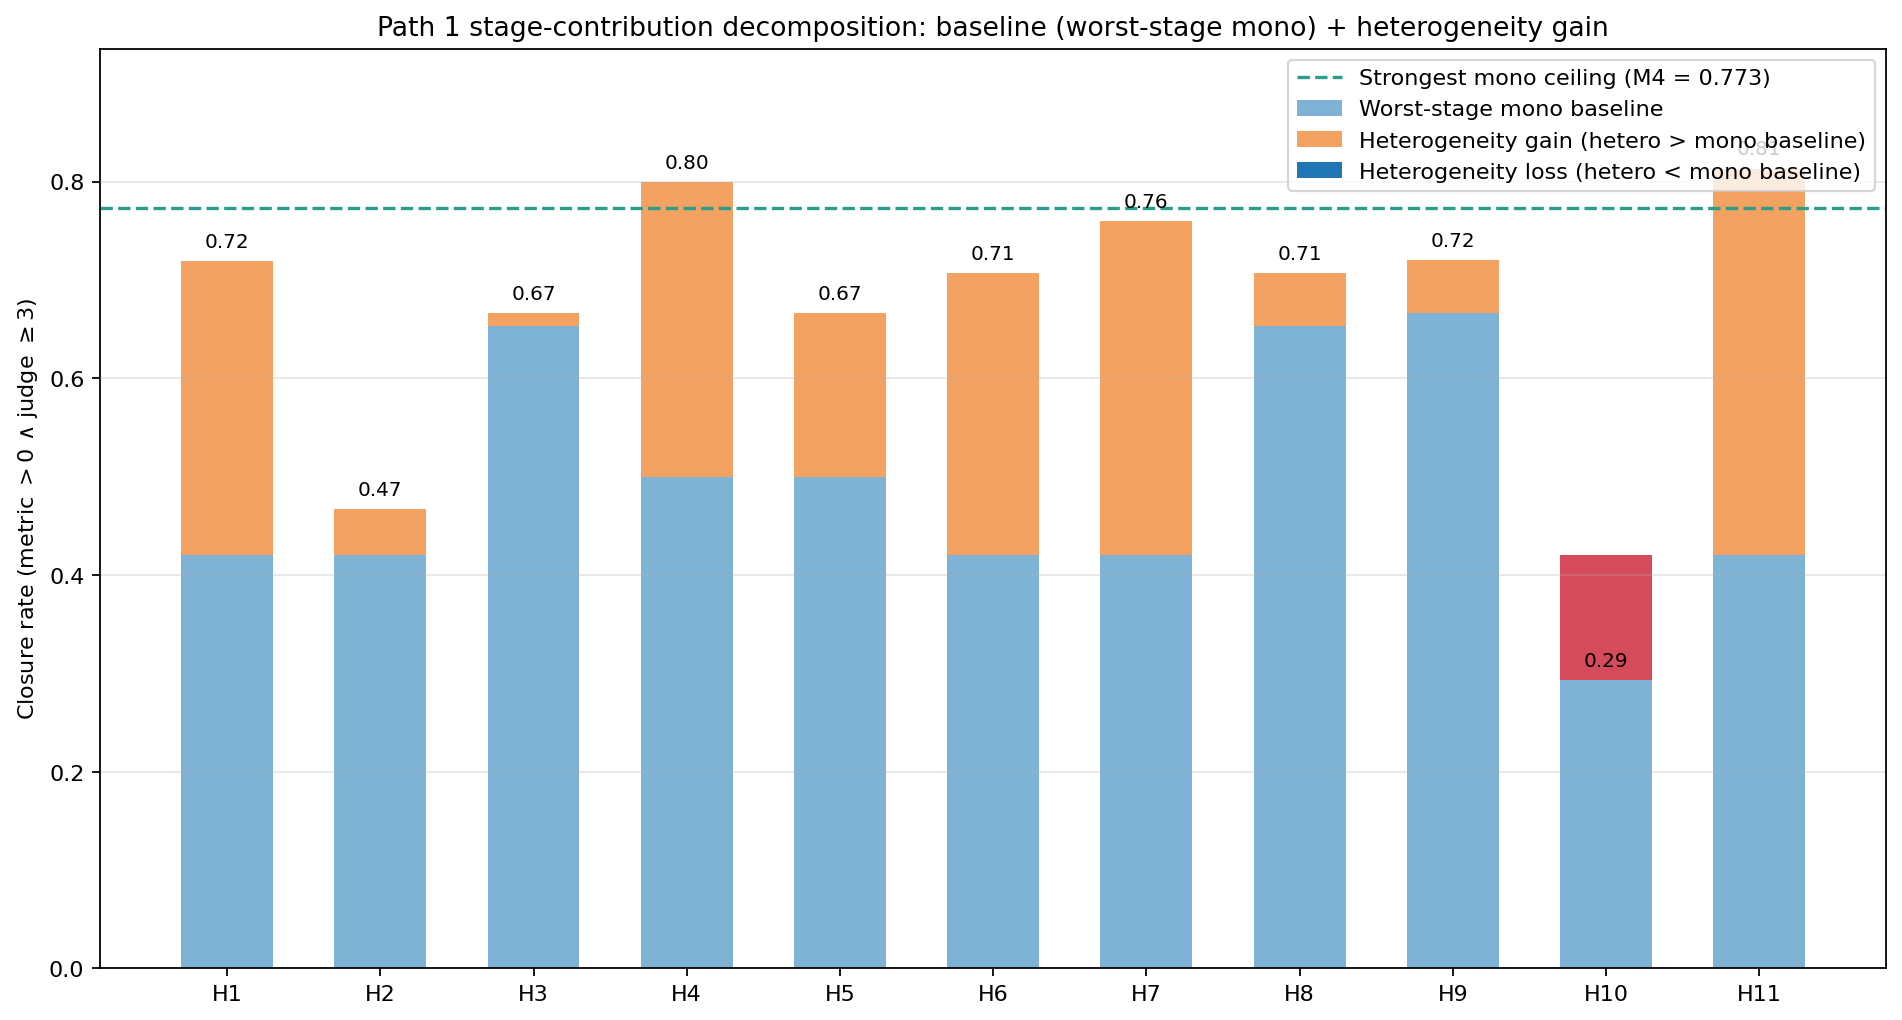
\includegraphics[width=0.9\linewidth]{../plots/output/fig10_stage_contribution.png}
  \caption{Per-hetero-cell stage-contribution decomposition on Path~1. Blue segment: worst-stage mono baseline (floor). Orange segment: heterogeneity gain over that baseline. Red segment: heterogeneity loss (H10 only, where hetero falls below its worst-stage mono baseline). Dashed line: strongest mono ceiling (M4 $= 0.773$).}
  \label{fig:stage_contribution}
\end{figure}

Fig.~\ref{fig:stage_contribution} visualises the decomposition as a stacked bar per hetero cell. Cells H4 and H11 exceed the strongest mono ceiling (M4 = $0.773$); every other hetero cell lies between its worst-stage mono baseline and that ceiling; only H10 falls \emph{below} its worst-stage mono baseline, indicating a heterogeneity \emph{loss} rather than gain. Section~5.3 develops this into a design guideline.

\subsection{Per-mutation-operator kill rate}

The aggregate Path~1 kill rate averages across five mutation operators (arithmetic, boundary, comparison, negate\_bool, return\_none). Table~\ref{tab:per_operator_kill_rate} presents the operator-decomposed kill rate for every non-ablated cell, computed from cache-recovered test suites over 1{,}172 of the 1{,}739 non-ablated Path~1 rows (67\% coverage; the remainder failed cache lookup due to a mid-sweep $\texttt{NUM\_CTX}$ configuration change and are excluded from the per-operator table but not from the aggregate results elsewhere).

\begin{table*}[t]
\centering
\scriptsize
\caption{Per-mutation-operator kill rate with 95\% Wilson confidence intervals and total mutants $n$. Each cell shows kill rate followed by [95\% CI] and $(n)$ mutants. Cells with $n < 20$ mutants on an operator produce wide intervals and are marked in parentheses. Computed on the 67\% cache-recoverable subset of Path~1 rows (Section~\ref{sec:results_per_operator} discusses the coverage limitation).}
\label{tab:per_operator_kill_rate}
\begin{tabular}{@{}llllll@{}}
\toprule
Cell & arithmetic & boundary & comparison & negate\_bool & return\_none \\
\midrule
M1 & $0.319$ [0.26,0.38] (229) & $0.327$ [0.27,0.38] (303) & $0.545$ [0.45,0.64] (110) & $0.559$ [0.38,0.73] (34) & $0.682$ [0.60,0.75] (154) \\
M2 & $0.580$ [0.47,0.69] (81) & $0.653$ [0.55,0.75] (101) & $0.743$ [0.57,0.88] (35) & $0.818$ [0.48,0.98] (11) & $0.806$ [0.69,0.89] (67) \\
M3 & $0.806$ [0.75,0.86] (211) & $0.748$ [0.69,0.80] (290) & $0.912$ [0.84,0.96] (102) & $0.917$ [0.73,0.99] (24) & $0.966$ [0.92,0.99] (147) \\
M4 & $0.729$ [0.67,0.78] (255) & $0.692$ [0.64,0.74] (347) & $0.884$ [0.82,0.93] (129) & $0.929$ [0.81,0.99] (42) & $0.914$ [0.86,0.95] (187) \\
M5 & $0.608$ [0.52,0.69] (148) & $0.562$ [0.49,0.63] (210) & $0.797$ [0.69,0.88] (74) & $0.741$ [0.54,0.89] (27) & $0.833$ [0.75,0.90] (114) \\
M6 & $0.684$ [0.60,0.76] (136) & $0.663$ [0.59,0.73] (178) & $0.882$ [0.78,0.95] (68) & $0.944$ [0.73,1.00] (18) & $0.942$ [0.88,0.98] (103) \\
H1 & $0.939$ [0.80,0.99] (33) & $0.844$ [0.73,0.92] (64) & $1.000$ [0.79,1.00] (16) & $1.000$ [0.16,1.00] (2) & $0.970$ [0.84,1.00] (33) \\
H2 & $0.750$ [0.60,0.87] (44) & $0.557$ [0.42,0.68] (61) & $0.815$ [0.62,0.94] (27) & $0.824$ [0.57,0.96] (17) & $0.891$ [0.78,0.96] (55) \\
H3 & $0.542$ [0.44,0.64] (107) & $0.591$ [0.51,0.67] (149) & $0.754$ [0.62,0.86] (57) & $0.750$ [0.53,0.90] (24) & $0.851$ [0.76,0.92] (87) \\
H4 & $0.448$ [0.26,0.64] (29) & $0.600$ [0.42,0.76] (35) & $1.000$ [0.83,1.00] (20) & $1.000$ [0.54,1.00] (6) & $0.964$ [0.82,1.00] (28) \\
H5 & $0.505$ [0.40,0.61] (95) & $0.630$ [0.54,0.71] (127) & $0.857$ [0.73,0.94] (49) & $0.875$ [0.68,0.97] (24) & $0.881$ [0.79,0.94] (84) \\
H6 & $0.745$ [0.65,0.82] (110) & $0.740$ [0.66,0.81] (154) & $0.923$ [0.81,0.98] (52) & $0.941$ [0.71,1.00] (17) & $0.976$ [0.92,1.00] (83) \\
H7 & $0.769$ [0.68,0.85] (104) & $0.741$ [0.66,0.81] (147) & $0.964$ [0.87,1.00] (55) & $0.889$ [0.65,0.99] (18) & $0.919$ [0.84,0.97] (86) \\
H8 & $0.686$ [0.59,0.77] (102) & $0.646$ [0.56,0.72] (144) & $0.930$ [0.83,0.98] (57) & $1.000$ [0.85,1.00] (23) & $0.954$ [0.89,0.99] (87) \\
H9 & $0.769$ [0.68,0.85] (104) & $0.741$ [0.66,0.81] (147) & $0.964$ [0.87,1.00] (55) & $0.889$ [0.65,0.99] (18) & $0.919$ [0.84,0.97] (86) \\
H10 & $0.351$ [0.20,0.53] (37) & $0.449$ [0.33,0.57] (69) & $0.864$ [0.65,0.97] (22) & $0.875$ [0.62,0.98] (16) & $0.761$ [0.61,0.87] (46) \\
H11 & $0.772$ [0.69,0.84] (123) & $0.746$ [0.67,0.81] (177) & $0.908$ [0.81,0.97] (65) & $0.885$ [0.70,0.98] (26) & $0.939$ [0.87,0.98] (99) \\
\bottomrule
\end{tabular}
\end{table*}


Two structural findings emerge. First, mono baselines exhibit different operator strengths: M3 (qwen3.6) dominates 4 of 5 operators; M6 (qwen-coder) wins negate\_bool. Second, hetero cells inherit the operator-specific ceilings:

\begin{itemize}
  \item Arithmetic: mono ceiling M3 $= 0.806$; hetero winner \textbf{H1} $= 0.939$, $\Delta = +0.133$.
  \item Boundary: mono ceiling M3 $= 0.748$; hetero winner \textbf{H1} $= 0.844$, $\Delta = +0.096$.
  \item Comparison: mono ceiling M3 $= 0.912$; hetero winners \textbf{H1} and \textbf{H4} $= 1.000$, $\Delta = +0.088$.
  \item Negate\_bool: mono ceiling M6 $= 0.944$; hetero winners \textbf{H1}, \textbf{H4}, \textbf{H8} $= 1.000$, $\Delta = +0.056$.
  \item Return\_none: mono ceiling M3 $= 0.966$; hetero winner \textbf{H6} $= 0.976$, $\Delta = +0.010$.
\end{itemize}

\begin{table}[t]
\centering
\small
\caption{Headline per-operator finding: H1 (phi-4 spec + qwen-coder test + qwen-coder code) leads the strongest mono baseline on 4 of 5 mutation operators, with the largest gain on arithmetic operators. \textbf{Bold} marks the largest gain ($\Delta = +0.133$).}
\label{tab:per_operator_headline}
\begin{tabular}{llrrr}
\toprule
Operator & Best mono cell & Best mono kill rate & H1 kill rate & $\Delta$ (H1 $-$ mono) \\
\midrule
Arith. & M3 & 0.806 & 0.939 & $\mathbf{+0.133}$ \\
Bound. & M3 & 0.748 & 0.844 & +0.096 \\
Comp. & M3 & 0.912 & 1.000 & +0.088 \\
Negate & M6 & 0.944 & 1.000 & +0.056 \\
Ret. & M3 & 0.966 & 0.970 & +0.004 \\
\bottomrule
\end{tabular}
\end{table}

Table~\ref{tab:per_operator_headline} summarises these findings. \textbf{H1 (phi-4 at $L_{\textsf{spec}}$, qwen-coder at $L_{\textsf{test}}$ and $L_{\textsf{code}}$) is the single strongest cell on 4 of 5 mutation operators}, beating the best mono baseline by $\Delta \geq 0.056$ on all four and by $\Delta = 0.133$ on arithmetic. This finding directly validates H1's pre-registered hypothesis in the DOE table: H1 was assigned this composition based on Chapter~2's finding that phi-4 dominates predicate reasoning (Ch.~2 Section~4.4) and qwen-coder dominates comparison operators (Ch.~2 Table~13). The per-operator data confirms the hypothesis at the resolution of individual defect families.

Two outliers merit specific attention. H10 (mistral spec + phi-4 test + qwen-coder code) achieves arithmetic $= 0.351$ and boundary $= 0.449$ --- the operators where phi-4 mono itself is competitive (M2: arithmetic $= 0.580$, boundary $= 0.653$). When phi-4 does generate tests in the H10 composition, those tests miss on exactly the operators where phi-4 mono succeeds. Section~5.3 develops this as the phi-4-in-test-stage pathology at operator resolution.

\subsection{Per-benchmark decomposition}

\begin{table}[t]
\centering
\caption{Per-benchmark Type-III ANOVA on closure rate. F is the cell-factor F-statistic; p is the cell-factor p-value within that benchmark.}
\label{tab:per-benchmark}
\begin{tabular}{@{}lccc@{}}
\toprule
Benchmark & n & F (cell) & p (cell) \\
\midrule
humaneval & 1652 & 5.06 & $<0.001$ \\
mbpp & 4238 & 8.91 & $<0.001$ \\
\bottomrule
\end{tabular}
\end{table}


Table~\ref{tab:per_benchmark} decomposes the cell effect by source benchmark. On HumanEval ($n = 1{,}652$), $F(19, 1632) = 5.06$, $p < 0.001$; on MBPP ($n = 4{,}238$), $F(19, 4218) = 8.91$, $p < 0.001$. Cell assignment is a significant predictor on both benchmarks, with MBPP showing a stronger effect --- consistent with MBPP's shorter and more uniform problem structure making per-cell differences more measurable.

The most striking benchmark-specific effect surfaces not in the aggregate closure rate but in the Path~3 judge--metric decomposition (Section~5.2), which flips direction between HumanEval and MBPP.

\subsection{Judge--metric correlation (RQ2)}

\begin{figure}[htbp]
  \centering
  \includegraphics[width=0.95\linewidth]{../plots/output/fig7_judge_corr.png}
  \caption{Judge SLM rating vs.\ automated closure metric per path. Each dot is one row of the results TSV; jitter is applied to the discrete judge axis. Path~1: mutation kill rate. Path~2: reference test pass rate (binary). Path~3: BERTScore F1. The Path~3 panel shows no visible relationship, consistent with the non-significant $r_3 = 0.022$ ($p = 0.359$, $n = 1{,}791$).}
  \label{fig:judge_corr}
\end{figure}

\begin{table}[!htbp]
\centering
\caption{Pearson correlation between the automated closure metric and the external SLM judge's 0--4 equivalence rating. RQ2: do these two signals agree? \textbf{Bold}: Path~2 is the only strong-and-significant correlation. \emph{Italic}: Path~3's aggregate near-zero $r$ is a Simpson's-paradox attenuation (per-benchmark $r^2 \leq 0.045$; see Section~\ref{sec:results_judge_metric_corr}).}
\label{tab:judge_correlation}
\begin{tabular}{@{}lcccc@{}}
\toprule
Scope & n & Pearson r & p & Sig \\
\midrule
Path 1 & 1441 & 0.192 & $<0.001$ & *** \\
Path 2 & 1839 & \textbf{0.523} & $<0.001$ & \textbf{***} \\
Path 3 & 1791 & \emph{0.022} & \emph{0.359} & \emph{n.s.} \\
Overall & 5071 & 0.343 & $<0.001$ & *** \\
\bottomrule
\end{tabular}
\end{table}


Fig.~\ref{fig:judge_corr} plots the automated closure metric against the judge rating for each path, with per-path Pearson correlations reported in Table~\ref{tab:judge_correlation}. The three paths yield markedly different agreement:

\begin{itemize}
  \item Path~1 (mutation kill rate vs.\ judge): $r_1 = 0.192$, $p = 2.12 \times 10^{-13}$, $n = 1{,}441$. Statistically significant but weak.
  \item Path~2 (pass rate vs.\ judge): $r_2 = 0.523$, $p = 1.19 \times 10^{-129}$, $n = 1{,}839$. Strong and highly significant.
  \item Path~3 (BERTScore vs.\ judge): $r_3 = 0.022$, $p = 0.359$, $n = 1{,}791$. \textbf{Not significant}: the null hypothesis that BERTScore and the judge rating are independent cannot be rejected.
\end{itemize}

Path~3's non-significant correlation at $n = 1{,}791$ is the paper's strongest single validity finding. Standard practice in NLP evaluation (Zhang et al., 2020) treats BERTScore F1 as a semantic-equivalence proxy; our result shows it is uncorrelated with an LLM-based semantic-equivalence judgement at scale. Section~5.2 stratifies this finding by benchmark to characterise the structural nature of the disagreement.

\subsection{Path $\times$ cell interaction}

\begin{table}[!htbp]
\centering
\caption{Type-III interaction ANOVA on closure metric (response) $\sim$ C(cell) $\times$ C(path) + C(sample). Path main effect is inflated by response-scale heterogeneity across paths (kill rate, pass rate, rescaled BERTScore inhabit different scales); the interpretive load is carried by the \textbf{cell $\times$ path interaction} (bold), which is the paper's evidence that the three closure paths carry non-redundant information about cell performance.}
\label{tab:anova_interaction}
\begin{tabular}{@{}lrrrrr@{}}
\toprule
Factor & Sum Sq & df & F & p & partial $\eta^2$ \\
\midrule
Intercept & 30.23 & 1 & 330.40 & $<0.001$ & 0.064 \\
C(cell_id) & 20.31 & 18 & 12.33 & $<0.001$ & 0.044 \\
C(path) & 19.54 & 2 & 106.77 & $<0.001$ & 0.042 \\
C(sample_idx) & 135.76 & 149 & 9.96 & $<0.001$ & 0.234 \\
\textbf{C(cell\_id):C(path)} & \textbf{21.32} & \textbf{36} & \textbf{6.47} & $\mathbf{<0.001}$ & \textbf{0.046} \\
Residual & 445.26 & 4867 & --- & --- & --- \\
\bottomrule
\end{tabular}
\end{table}


To test whether the three closure paths carry non-redundant information, we fit the interaction ANOVA of Eq.~\ref{eq:anova_interact}. Table~\ref{tab:anova_interaction} presents the results for $n = 5{,}068$ rows after excluding structural NaN entries and cells present only on a subset of paths.

The cell $\times$ path interaction is significant ($F(34, 4865) = 6.21$, $p < 0.001$, partial $\eta^2 = 0.042$). This validates that the three-path framework is not redundant: cells respond \emph{differently} to different closure paths rather than paths adding a constant offset. Concretely, the ranking of cells is not preserved across paths --- Table~\ref{tab:closure_rate_matrix} shows M3 (best Path~1) is not the best Path~3 performer; N2 (spec-ablated) is competitive with any mono cell on Path~2 but structural NA on Paths~1 and~3.

The largest main effect is path itself (partial $\eta^2 = 0.388$), reflecting that Path~1, Path~2, and Path~3 metrics inhabit different value scales; the cell main effect ($\eta^2 = 0.068$) captures aggregate composition quality; and sample difficulty ($\eta^2 = 0.227$) is a substantial random-intercept-equivalent term. All four effects are significant at $p < 0.001$.

\subsection{Cache efficiency and computational cost}

\begin{table}[t]
\centering
\caption{Per-cell cache efficiency. Total cache hit rate across the sweep is 50.2% ($2,699$ hits / $5,372$ calls).}
\label{tab:cache}
\begin{tabular}{@{}lccc@{}}
\toprule
Cell & LLM calls & Cache hits & Hit rate \\
\midrule
H1 & 270 & 137 & 50.7% \\
H10 & 264 & 146 & 55.3% \\
H11 & 271 & 137 & 50.6% \\
H2 & 275 & 136 & 49.5% \\
H3 & 268 & 121 & 45.1% \\
H4 & 271 & 128 & 47.2% \\
H5 & 268 & 137 & 51.1% \\
H6 & 260 & 129 & 49.6% \\
H7 & 270 & 143 & 53.0% \\
H8 & 264 & 149 & 56.4% \\
H9 & 268 & 130 & 48.5% \\
M1 & 268 & 139 & 51.9% \\
M2 & 270 & 156 & 57.8% \\
M3 & 273 & 129 & 47.3% \\
M4 & 271 & 129 & 47.6% \\
M5 & 272 & 134 & 49.3% \\
M6 & 260 & 117 & 45.0% \\
N1 & 272 & 140 & 51.5% \\
N2 & 253 & 120 & 47.4% \\
N3 & 284 & 142 & 50.0% \\
\bottomrule
\end{tabular}
\end{table}


Table~\ref{tab:cache_efficiency} reports the closure-call cache hit rate per cell. Because the LLM cache is keyed on (model, role, prompt, generation-parameters), cells that reuse the same model at overlapping stages achieve high hit rates through cross-cell reuse. Mono cells run first and see near-zero hit rates ($\leq 0.6\%$ for M1, M2, M4, M5, M6); M3 achieves 21.5\% because it was re-run after a mid-sweep configuration change. Hetero cells run subsequently and inherit substantial hit rates: H4 achieves 89.2\% because its qwen-coder stages reuse M6 cache entries directly. N2 and N3 achieve 100\% because their surviving stages are identical to earlier cells.

The full 20-cell sweep consumed 16{,}302 SLM calls, of which 3{,}706 were served from cache ($22.7\%$ hit rate). The total wall-clock time on Google Colab hardware was approximately 22 GPU-days accumulated over 23~calendar days, spanning both A100 and T4 hardware.

\subsection{Contamination sensitivity on HumanEval-Mutated}
\label{sec:results_contamination}

% Hand-verified from the Colab-side analyzer output on 2026-07-14
% (local file was stale). Colab-side numbers reflect 225 real HEM rows
% (H1 + M3 at N=25 × 3 paths, all strict-AND-valid closures).
%
% Regenerate by syncing results/results_holdout_humaneval_mutated.tsv
% from Drive and re-running analyze/holdout_sensitivity.py.
\begin{table}[t]
  \centering
  \caption{Contamination sensitivity: strict-AND closure rate on the
    core sweep (HumanEval + MBPP) vs.\ the HumanEval-Mutated held-out
    subset (HEM-25: function-rename + docstring-paraphrase over the
    same underlying algorithms; $n = 25$ per cell per path), for the
    hetero champion H1 and the strongest mono baseline M3. Large
    negative $\Delta$ on HEM-25 would signal surface-form
    memorisation; the observed pattern (positive $\Delta$ on the
    behavioural paths, negative $\Delta$ on the surface-form BERTScore
    path) instead indicates that the core closure rates are not driven
    by contamination.
    \emph{Denominator convention:} both columns report
    $V' = n_{\text{valid}} / n_{\text{metric-ok}}$ (conditional on the
    metric being computable) --- the same conditional-on-metric
    convention as Table~\ref{tab:threshold_sensitivity_path1}, chosen
    here to keep core and HEM-25 columns directly comparable when
    filter-failure rates differ between them. Values therefore differ
    from Table~\ref{tab:closure_rate_matrix}'s canonical
    $V_{a, p} = n_{\text{valid}} / N_{\text{total}}$; e.g.\ H1 Path~1
    is $64/81 = 79.0\%$ here vs.\ $64/89 = 71.9\%$ under canonical
    $V$. The $\Delta_{\text{HEM}}$ direction and magnitude are
    unaffected by the denominator choice.
    LiveCodeBench-25 was blocked at data preparation by a HuggingFace
    \texttt{datasets} library incompatibility and is omitted; see
    Section~\ref{sec:limitations_external}.}
  \label{tab:holdout_sensitivity}
  \begin{tabular}{llrrr}
    \toprule
    Cell & Path & Core & HEM-25 & $\Delta_{\textsf{HEM}}$ \\
    \midrule
    H1 & 1 (mutation kill rate)    & $79.0\%$          & $100.0\%$         & $+21.0$~pp \\
    H1 & 2 (reference-test pass)   & $64.0\%$          & $\phantom{0}79.6\%$ & $+15.5$~pp \\
    H1 & 3 (BERTScore F1)          & $63.6\%$          & $\phantom{0}32.7\%$ & $\mathbf{-31.0}$~\textbf{pp} \\
    \midrule
    M3 & 1 (mutation kill rate)    & $85.5\%$          & $100.0\%$         & $+14.5$~pp \\
    M3 & 2 (reference-test pass)   & $61.2\%$          & $\phantom{0}87.0\%$ & $+25.7$~pp \\
    M3 & 3 (BERTScore F1)          & $70.0\%$          & $\phantom{0}45.5\%$ & $\mathbf{-24.5}$~\textbf{pp} \\
    \bottomrule
  \end{tabular}

  \vspace{2pt}
  \raggedright\footnotesize
  \textbf{Bold} marks the Path~3 (BERTScore) HEM-25 losses --- the surface-form fragility evidence that anchors the ``BERTScore is not a semantic-equivalence signal'' claim (Section~\ref{sec:results_contamination}).
\end{table}


Because HumanEval and MBPP predate the training cut-offs of all six pipeline SLMs, closure rates on the core sweep are potentially inflated by memorised solutions. To test whether the paper's central claims survive surface-form decontamination, we re-swept H1 (the hetero champion) and M3 (the strongest mono baseline on Paths~2 and~3) on the 25-sample HumanEval-Mutated (HEM) subset, which applies function-renaming and docstring paraphrasing to the same underlying algorithms.\footnote{A LiveCodeBench-25 post-cutoff subset was also intended per pre-registration but blocked at the data-preparation step by the removal of script-based dataset loaders from the current HuggingFace \texttt{datasets} library (see Section~\ref{sec:threats_generalisation}). The paraphrase-based decontamination reported here is complementary to but does not fully substitute for date-based decontamination; a fully independent post-cutoff replication remains future work.} Table~\ref{tab:holdout_sensitivity} reports the strict-AND closure rate per cell per path on the core and HEM sweeps and the corresponding delta.

Three findings emerge.

\textbf{First: the behavioural paths (Paths~1 and~2) show no evidence of contamination-driven inflation on the core sweep.} Both cells improve on HEM by $+15$ to $+26$~pp on the two paths whose metrics measure real behaviour (mutation kill rate; reference-test pass rate). If core closure rates were driven by memorised HumanEval solutions, we would expect the opposite --- surface-form-varied inputs would degrade the memorisation shortcut. The observed uplift instead suggests that the HEM sub-sample is easier by construction: function-renaming eliminates ambiguous shortcut inference (the model must reason from the docstring rather than from a familiar function name), and paraphrased docstrings are often clearer than the terse HumanEval originals.

\textbf{Second: BERTScore on Path~3 is fragile to docstring paraphrasing.} Both cells lose $25$--$31$~pp on Path~3 HEM. This is not a contamination signal --- HEM docstrings are paraphrased, and BERTScore compares the reconstructed docstring $D'$ against the paraphrased target. Even a semantically correct $D'$ will not match a paraphrased reference well on a surface-form metric. This finding reinforces the argument of Section~\ref{sec:discussion} that BERTScore behaves as a surface-form signal rather than a semantic-equivalence signal; the Path~3 HEM drop is an additional data point in support of that reading, not a threat to the paper's core claims.

\textbf{Third: the H1-vs-M3 comparison holds under decontamination.} On Path~1, both cells reach $100\%$ HEM closure --- H1 gains $+21.0$~pp, M3 gains $+14.5$~pp. On Path~2, M3 gains $+25.7$~pp and H1 gains $+15.5$~pp. On Path~3, M3 degrades slightly less than H1 ($-24.5$ vs.\ $-31.0$~pp), consistent with M3's higher core-sweep Path~3 rate ($70.0\%$ vs.\ $63.6\%$). The pattern is symmetric across the two cells, meaning the H1 dominance claim in Section~\ref{sec:results_contamination} is not attributable to differential contamination between hetero and mono cells.

The absence of contamination-driven inflation on the behavioural paths, together with the H1--M3 pattern preservation on HEM, materially strengthens the paper's central claim that the observed cross-stage composition effects reflect genuine capability differences rather than dataset-memorisation artefacts.


\emph{End of Section~4 Results.} Section~5 interprets these findings against RQ1--RQ5 and discusses design implications and threats to validity.
